\chapter{Progettazione} \label{chapter:prog}
In questo capitolo si andranno ad esporre quelle che sono state le scelte di progettazione per l'implementazione del software oggetto di questa relazione. In particolare verranno discusse le scelte tecniche per ciò che concerne la progettazione del client e del server, nonché le scelte sulle tecnologie utilizzate
Quest'ultime vengono descritte dettagliatamente nell'appendice \ref{appendix:a}.\\

Il software in questione è stato pensato per essere scalabile, mantenibile ed integrabile, eventualmente, con altri sistemi già esistenti. Per tale ragione si è deciso di adottare un'architettura software suddivisa in vari livelli, utilizzando in particolare il pattern \textit{Model View Controller} (MVC) introdotto nel capitolo \ref{chapter:intro}, sia lato client che lato server. Mentre per ciò che riguarda i servizi web, si è scelto di utilizzare un'architettura REST (anche questo concetto è stato introdotto nel capitolo \ref{chapter:intro}), implementando una API (\textit{Application Programming Interface}) lato server e accedendo quindi alle risorse mediante protocollo HTTP (\textit{Hypertext Transfer Protocol}). In particolare si tratta di una API che restituisce i dati richiesti in formato JSON (\textit{JavaScript Object Notation}), un'alternativa al classico XML (\textit{Extensible Markup Language}). Questa scelta deriva dal fatto che tale formato è di semplice lettura, in quanto ha uno stile più compatto e intuitivo rispetto all'XML. Inoltre, il processo di analisi, ossia la velocità di interpretazione da parte di un computer, risulta essere più veloce rispetto all'altro linguaggio citato, e questo sempre dato dalla compattezza, dunque dall'utilizzo di meno dati per descrivere una risorsa. Infine, un ulteriore vantaggio è dato dal fatto che un oggetto JSON nella maggior parte dei casi corrisponde interamente agli oggetti dell'applicazione, ciò rende semplice e performante il \textit{binding} dei dati in entrambi i sensi (dal server al client e viceversa).  

\subsection{Client}
Lato client l'applicazione viene eseguita mediante web browser. Per l'implementazione si è scelto di utilizzare il framework Angular 8\aref{appendix:angular}, il quale è basato sul linguaggio TypeScript e adoperato per la creazione di applicazioni web \textit{single-page}. La scelta di tale framework deriva, appunto, dalla necessità di avere un'applicazione sviluppata in una singola pagina, costituita da vari componenti (o moduli), i quali vengono caricati dinamicamente a seconda delle azioni dell'utente e senza il bisogno di ricaricare una nuova pagina web, facendo un'ulteriore richiesta al server. Inoltre, l'uso di tale tecnologia rende del tutto indipendente il livello client dal livello server, basando la loro comunicazione esclusivamente sull'impiego di un'architettura REST. In particolare, questa comunicazione avviene usando il protocollo HTTP, sfruttando i quattro metodi \texttt{GET}, \texttt{POST}, \texttt{PUT} e \texttt{DELETE}, e servendosi di determinati \textit{endpoints}, ovvero delle URLs (\textit{Uniform Resource Locators}) messe a disposizione dall'API e mediante le quali è possibile accedere ai servizi forniti lato server e quindi alle risorse. \\
Una possibile alternativa sarebbe potuta essere React.js, una libreria JavaScript sviluppata e mantenuta da Facebook, la quale permette, in modo concettualmente simile, di sviluppare un'applicazione in singola pagina. Un punto a favore è sicuramente l'efficienza, che risulta maggiore rispetto ad Angular, tuttavia possiede diverse lacune in termini di funzionalità e completezza e talvolta è necessario l'utilizzo di ulteriori strumenti di terze parti, ad esempio per il servizio di routing fra componenti dell'applicazione.\\

\noindent 
Riguardo la struttura del codice lato \textit{front-end}, ossia lato client, come già precedentemente anticipato, viene adottata una struttura multi-livello, in particolare seguendo il paradigma MVC. Nello specifico si ha:
\begin{itemize}
    \item un livello controller per ogni classe principale: tale ruolo viene svolto dal componente stesso, il quale rappresenta un oggetto dell'applicazione;
    \item un livello service: contiene la logica di business e contiene le istruzioni per le chiamate HTTP;
    \item un livello per il modello: viene utilizzato per il \textit{binding} dei dati e quindi definisce la struttura di una specifica entità dell'applicazione.
\end{itemize}
\noindent
Ad esempio, considerando di dover rappresentare la lista degli impiegati si avrà quanto segue:
\begin{itemize}
    \item il componente che rappresenta gli impiegati è costituito dai seguenti files:
    \begin{itemize}
        \item impiegati.component.css, dove è possibile definire lo stile estetico del componente, una volta visualizzato dal browser;
        \item impiegati.component.html, definisce la struttura del componente che il browser dovrà visualizzare e insieme al precedente file va a costituire la vista dell'applicazione;
        \item impiegati.component.ts, il quale rappresenta il controller.
    \end{itemize}
    \item impiegato.service.ts, ossia il livello di servizio, dove vengono definite le chiamate HTTP e la logica di business;
    \item impiegato.ts, dove viene definita la struttura dell'entità impiegato, dunque gli attributi che lo caratterizzano.
\end{itemize}

\noindent
\textit{Nota}: il tipo di estensione ".ts" è associato ai file che contengono codice TypeScript.


\subsection{Intefaccia utente}
L'interfaccia è stata progettata adoperando il software Adobe XD (\textit{Experience Design}) e poi implementata mediante il framework Angular. L'obiettivo primario nella fase di progettazione è stato quello di ottenere un'interfaccia grafica il più intuitiva e semplice possibile. Per l'implementazione sono stati utilizzati i linguaggi HTML e CSS, rispettivamente per definire la struttura e lo stile grafico di ogni singolo componente, o in generale della pagina web. \\
Di seguito vengono mostrati alcuni esempi, in particolare la pagina di login e le pagine del timesheet con accesso manager ed impiegato.

\begin{figure}[H]
	\centering
	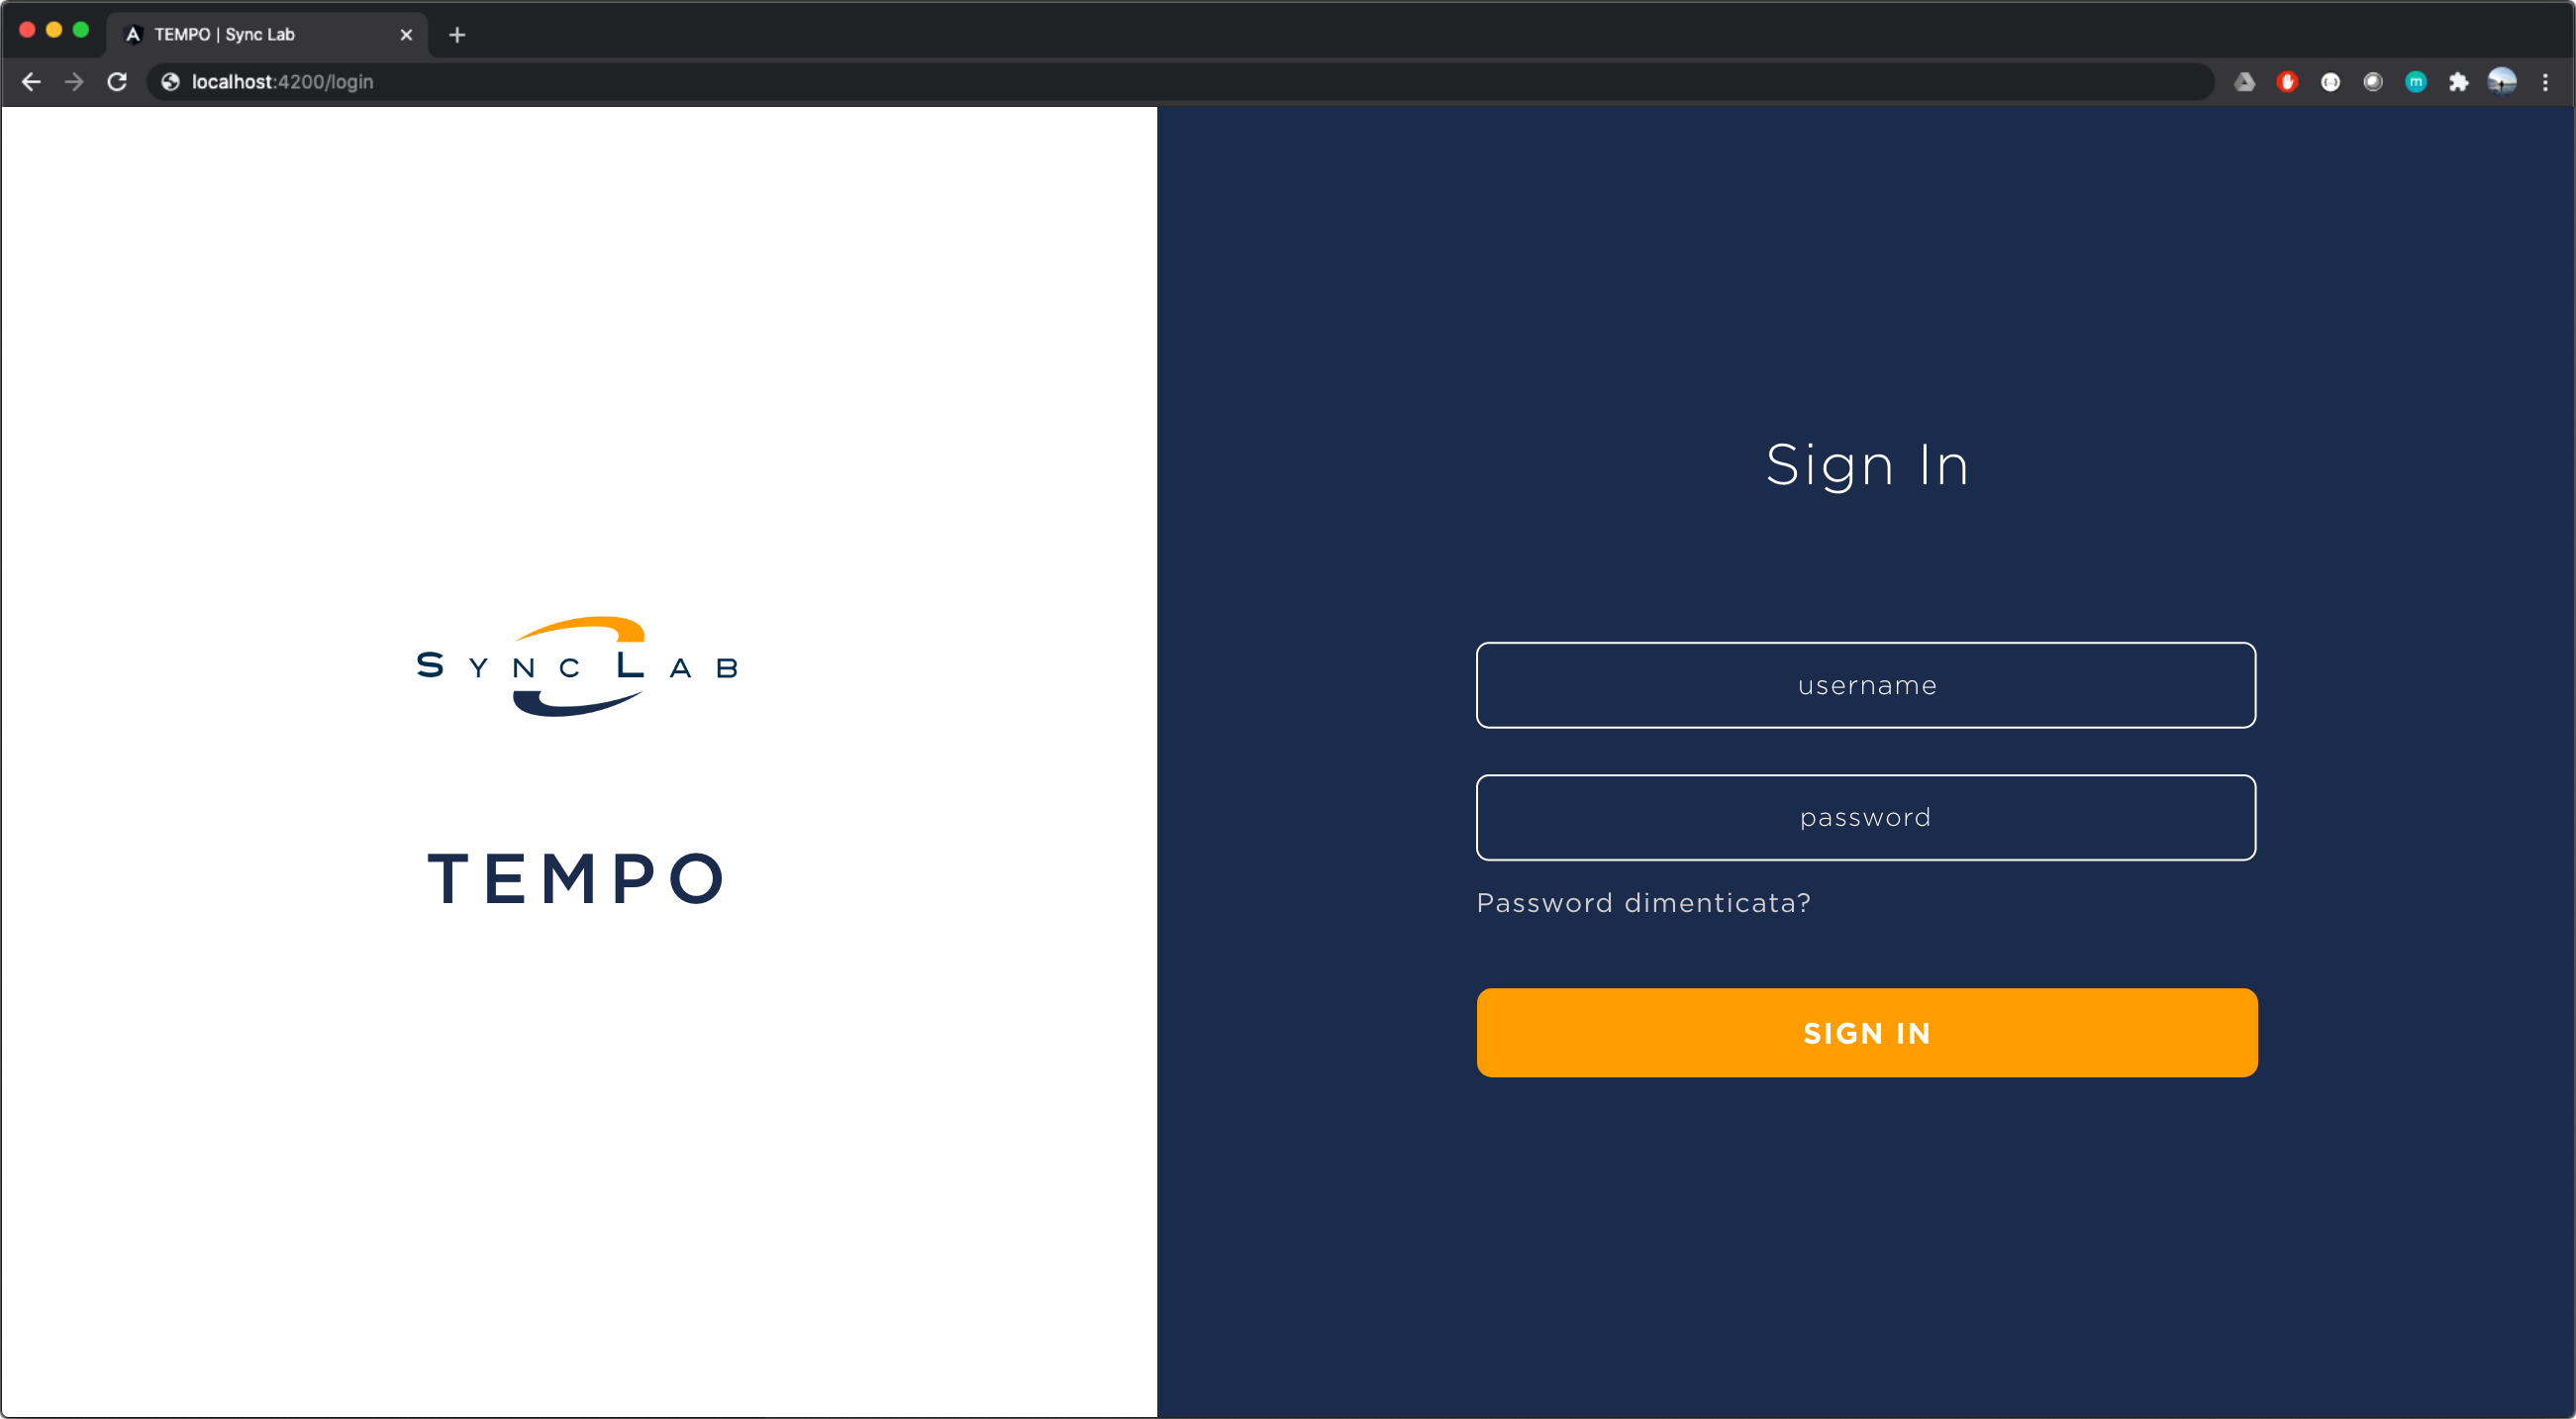
\includegraphics[width=1\textwidth]{login.png}
	\caption{Pagina di login.}	
	\label{fig:ui_login}
\end{figure}

\noindent
Osservando le figure \ref{fig:ui_manager} e \ref{fig:ui_impiegato}, è possibile notare funzionalità aggiuntive per l'utente manager. Precisamente, in figura \ref{fig:ui_manager}, sono presenti le sezioni "impiegati" e "risorse assegnate", che in figura \ref{fig:ui_impiegato} non compaiono. Tali funzionalità consentono al manager, rispettivamente, di gestire gli impiegati appartenenti alla sua sede e di gestire l'assegnamento di risorse a nuovi progetti, nonchè la creazione di nuovi codici commessa. Nella sezione archivio, vengono visualizzati i timesheet relativi ai mesi precedenti e si ha la possibilità di scaricarli in formato Excel.

\begin{figure}[H]
	\centering
	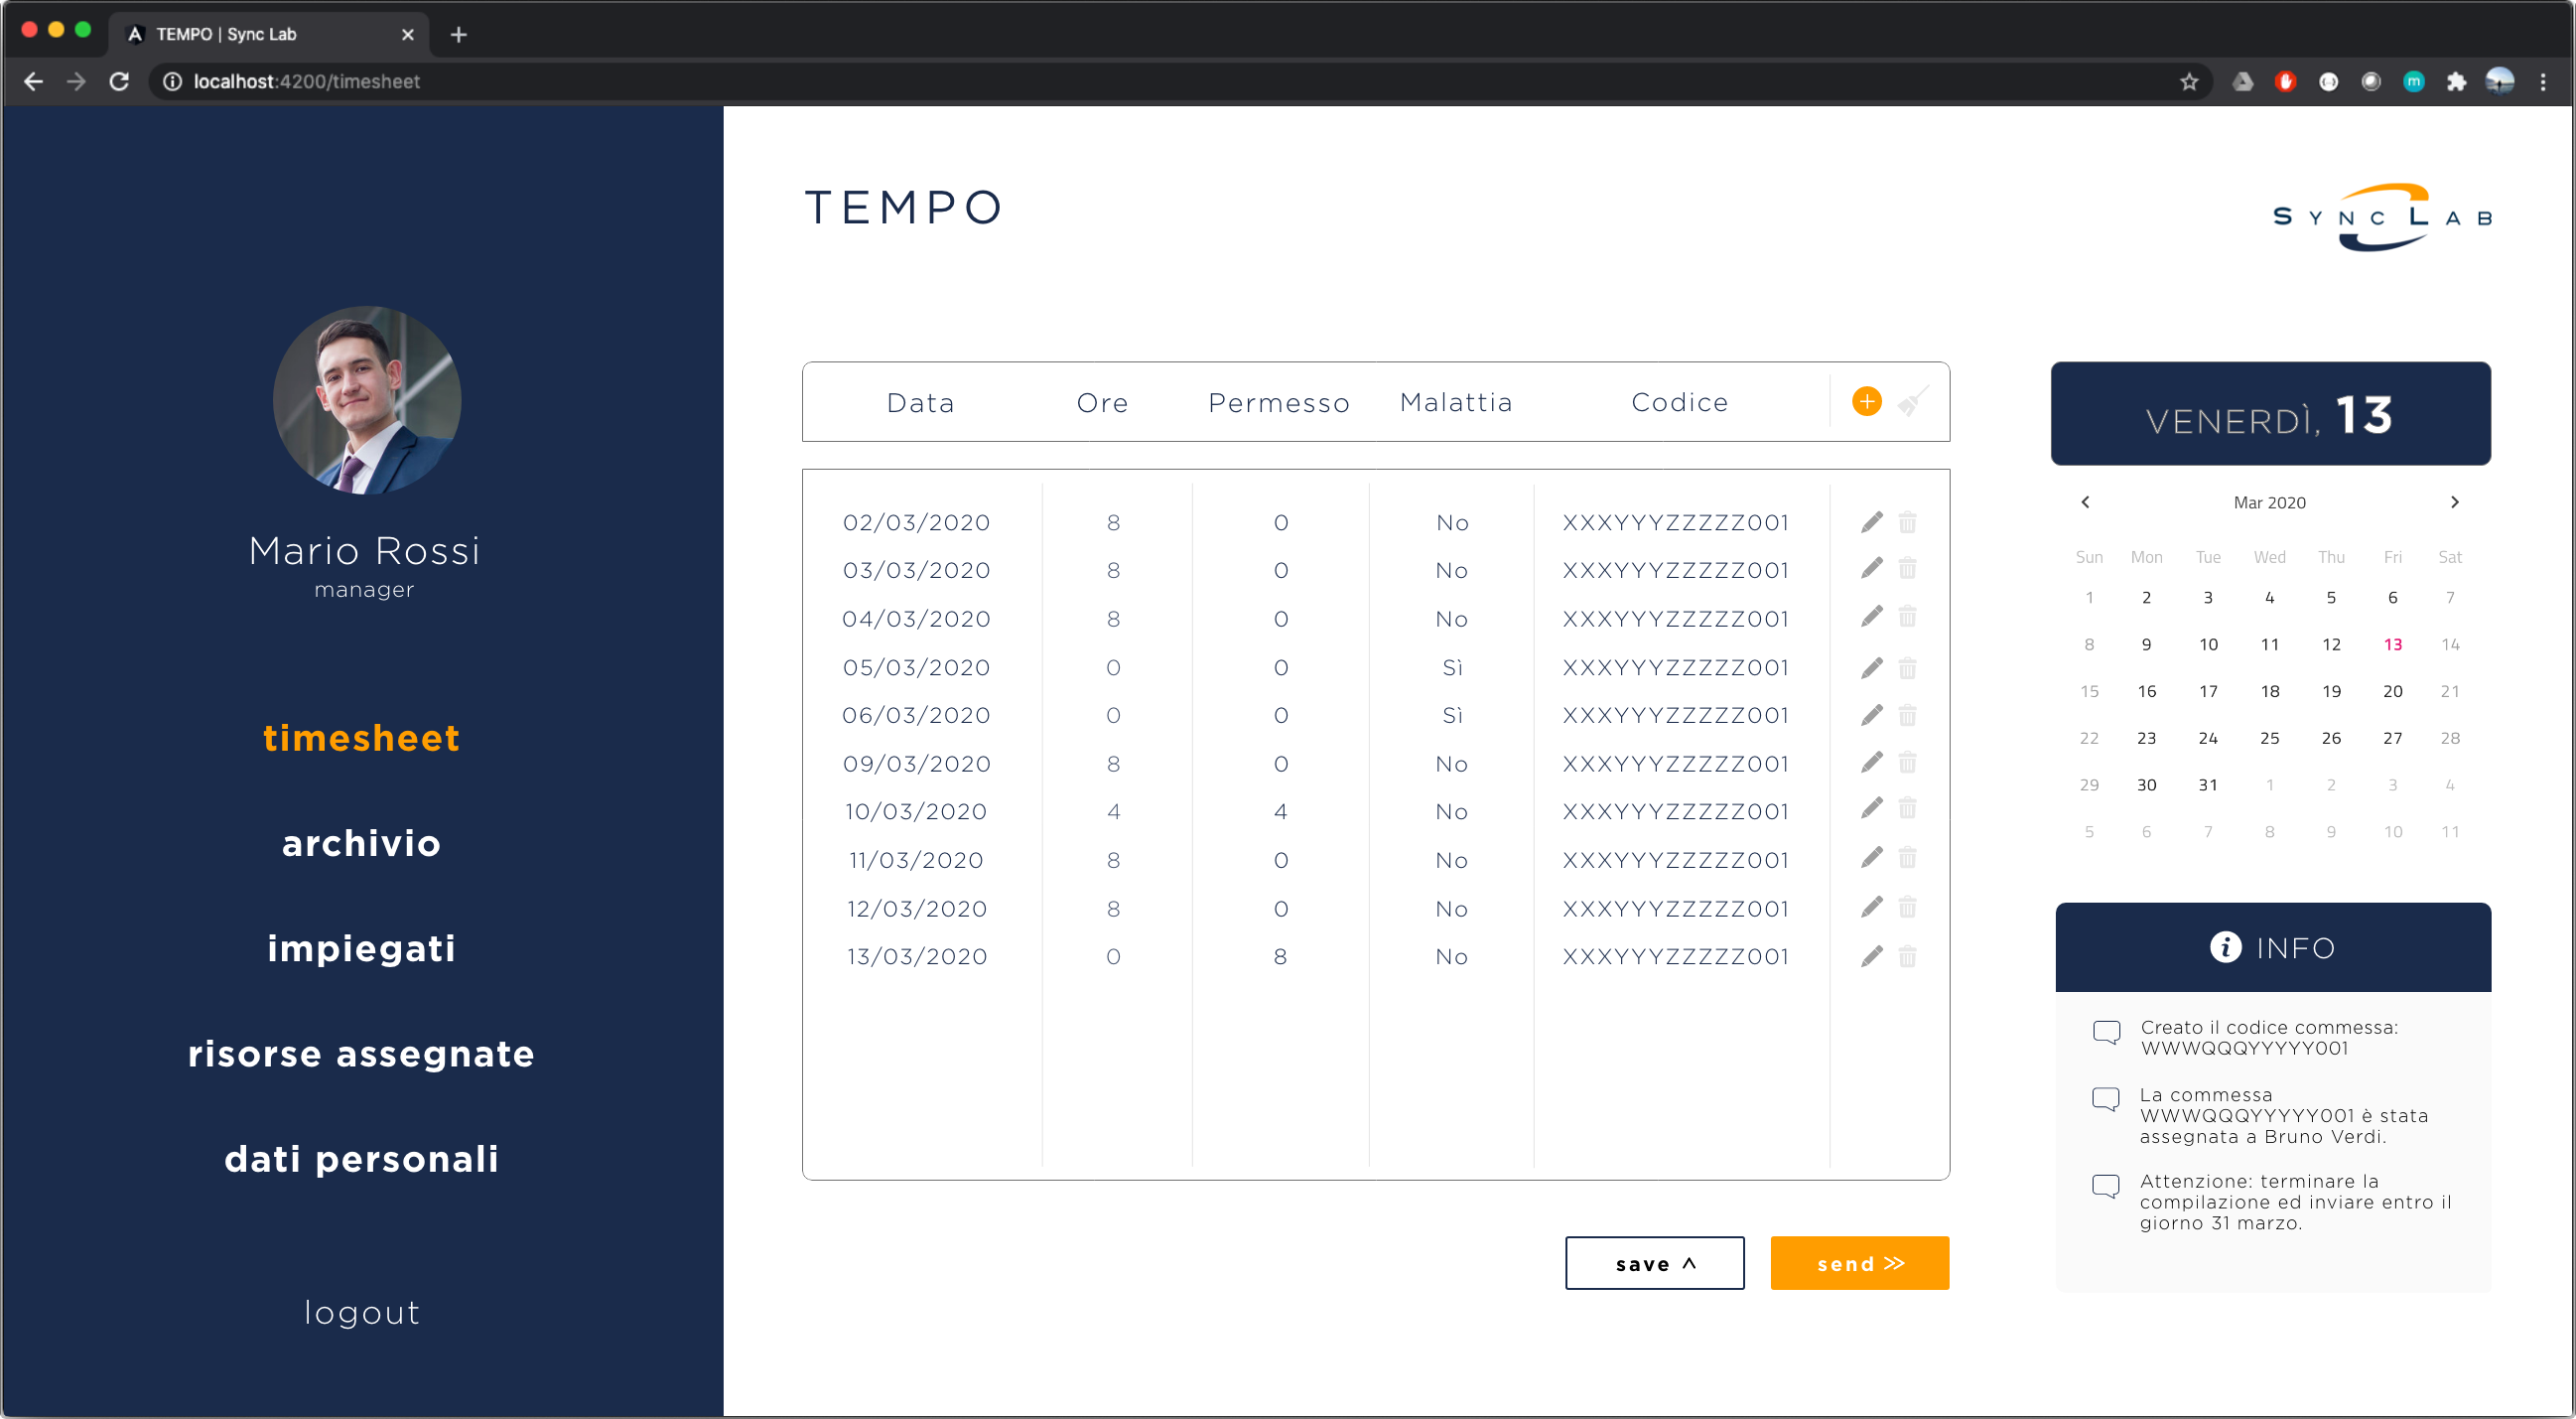
\includegraphics[width=1\textwidth ]{ui_manager.png}
	\caption{Sezione timesheet dell'interfaccia utente di un manager.}	
	\label{fig:ui_manager}
\end{figure}

\begin{figure}[H]
	\centering
	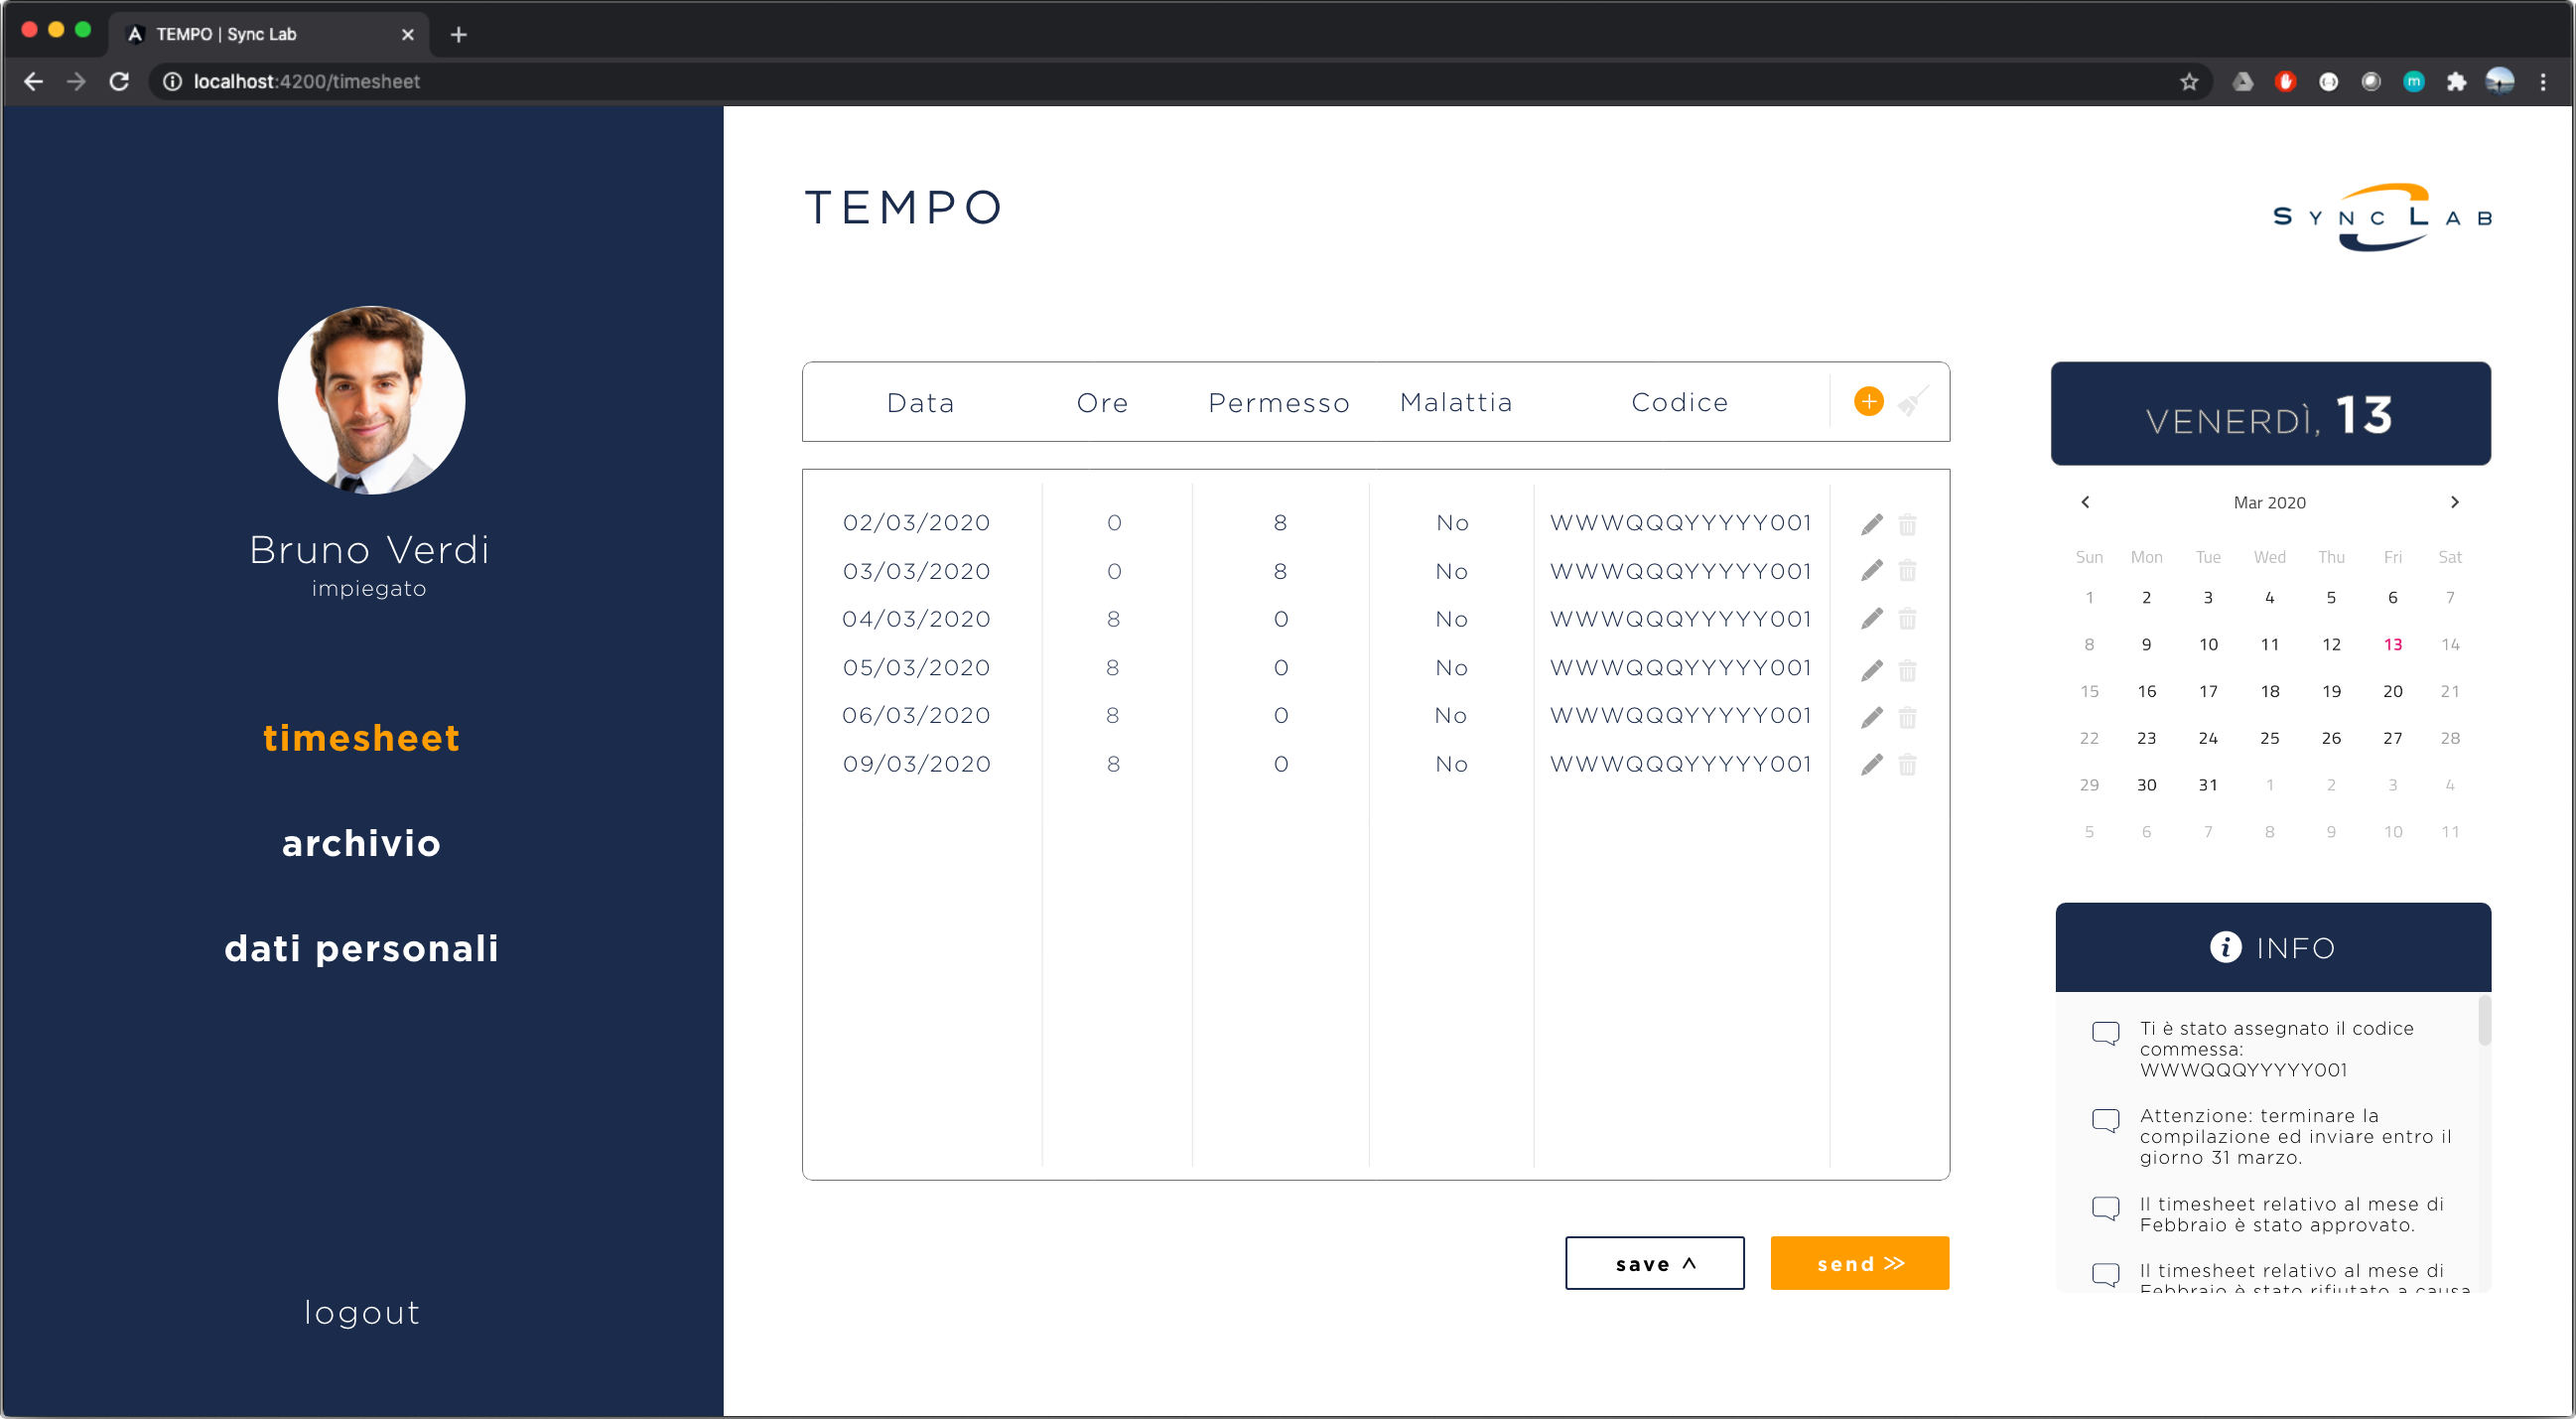
\includegraphics[width=1\textwidth]{ui_impiegato.png}
	\caption{Sezione timesheet dell'interfaccia utente di un impiegato.}	
	\label{fig:ui_impiegato}
\end{figure}

\subsection{Server}
Per quanto riguarda il server sono stati utilizzati i framework Spring\aref{appendix:spring}, in particolare Spring MVC, e Hibernate\aref{appendix:hibernate}, basati sul linguaggio di programmazione Java.

Spring è stato scelto poiché, oltre ad essere uno tra i più popolari framework per lo sviluppo di applicazioni Java Enterprise, permette di organizzare il codice secondo il pattern Model View Controller, citato in precedenza. Tale framework utilizza inoltre, il cosiddetto IoC (\textit{Inversion of Control}), ossia un principio di programmazione che consiste nell'assegnare il controllo del flusso del programma al framework stesso. Questo agevola la creazione di software modulare, riusabile e semplice, eventualmente, da estendere. Oltre a quanto già detto, mediante Spring è stato possibile implementare un'architettura REST grazie all'uso di specifiche annotazioni Java, messe a disposizione dal framework, e definendo inoltre gli endopoint necessari per la localizzazione delle risorse da parte del client, il quale potrà accedervi mediante richieste HTTP. 

In alternativa a Spring, si sarebbe potuto adoperare Struts, anch'esso un framework basato sul linguaggio Java e che permette la creazione di applicazioni web enterprise. In Struts, l'oggetto che si occupa di una richiesta e la instrada per l'ulteriore elaborazione è noto come \textit{Action} e sostanzialmente corrisponde a quello che in Spring viene chiamato \textit{Controller}. D'altra parte, Spring MVC è progettato attorno all'oggetto \textit{DispatcherServlet}, ossia un \textit{front controller}, responsabile della delegazione delle richieste agli specifici componenti (\textit{controller}) dell'applicazione. Dunque nel momento in cui si effettua una richiesta, questa viene presa in carico dal DispatcherServlet, il quale a sua volta l'assegnerà al controller di competenza che si preoccuperà dell'elaborazione. La differenza sostanziale in questa fase, sta nel fatto che in Struts viene inizializzato un oggetto Action, ogniqualvolta viene fatta una richiesta, mentre in Spring, i controller vengono inizializzati solo una volta e salvati in memoria, quindi sempre disponibili e condivisi tra le varie richieste, tale gestione offre una maggiore efficienza. Inoltre, un'ulteriore differenza riguarda la flessibilità sulla definizione degli oggetti che compongono l'applicazione: in Spring esiste una separazione dei ruoli, ben definita, tra Controller, Model e View, ma non vengono poste particolari restrizioni sulla definizione degli oggetti; al contrario Struts forza l'uso delle Actions e degli ActionForms. Infine la testabilità di un'applicazione sviluppata mediante Spring, grazie anche al concetto di IoC, risulta più semplice. Per tali ragioni si è deciso di utilizzare Spring Framework.

Per quanto concerne la persistenza dei dati, ossia la loro manipolazione, è stato usato il framework Hibernate. Esso offre una serie di servizi ad alte prestazioni, legati all'interazione tra un'applicazione Java e un database relazionale. Precisamente Hibernate è uno strumento per l'\textit{Object Relational Mapping} (ORM), ossia una tecnica di programmazione per il mappaggio delle classi Java alle tabelle di un database relazionale (e dati tipi Java ai tipi di dato del linguaggio SQL). 

\noindent
In aggiunta, fornisce funzionalità di query e recupero dei dati, in generale per la loro gestione e manipolazione. Questo è possibile poiché esso implementa quelle che sono le specifiche principali per ciò che riguarda la persistenza dei dati, ovvero quanto definito dalla \textit{Java Persistence API} (JPA). I principali vantaggi di Hibernate sono i seguenti: 
\begin{itemize}
    \item open source e di dimensioni contenute;
    \item alte prestazioni, grazie all'uso di un doppio livello di memoria cache implementate all'interno del framework;
    \item query indipendenti dal database, questo grazie al linguaggio \textit{Hibernate Query Language} (HQL), ossia una versione orientata agli oggetti del linguaggio SQL;
    \item creazione automatica delle tabelle del database, dunque non c'è la necessità di doverle creare manualmente.
\end{itemize}

\noindent
Nello specifico, il codice è stato strutturato su tre livelli:
\begin{itemize}
    \item Controller, il quale si occupa di reindirizzare le richieste provenieti dal client e recuperare i dati richiesti usufruendo del livello service.
    \item Service, contenente la logica di business dell'applicazione.
    \item Model, costituito da due ulteriori livelli: 
    \begin{itemize}
        \item DAO (\textit{Data Access Object}), il quale contiene i metodi, implementati mediante l'uso del framework Hibernate, per la manipolazione dei dati.
        \item Entity, il quale definisce la struttura delle entità che compongono l'applicazione.
    \end{itemize}
\end{itemize}

\clearpage
\section{Diagramma delle classi}
\begin{figure}[H]
	\centering
	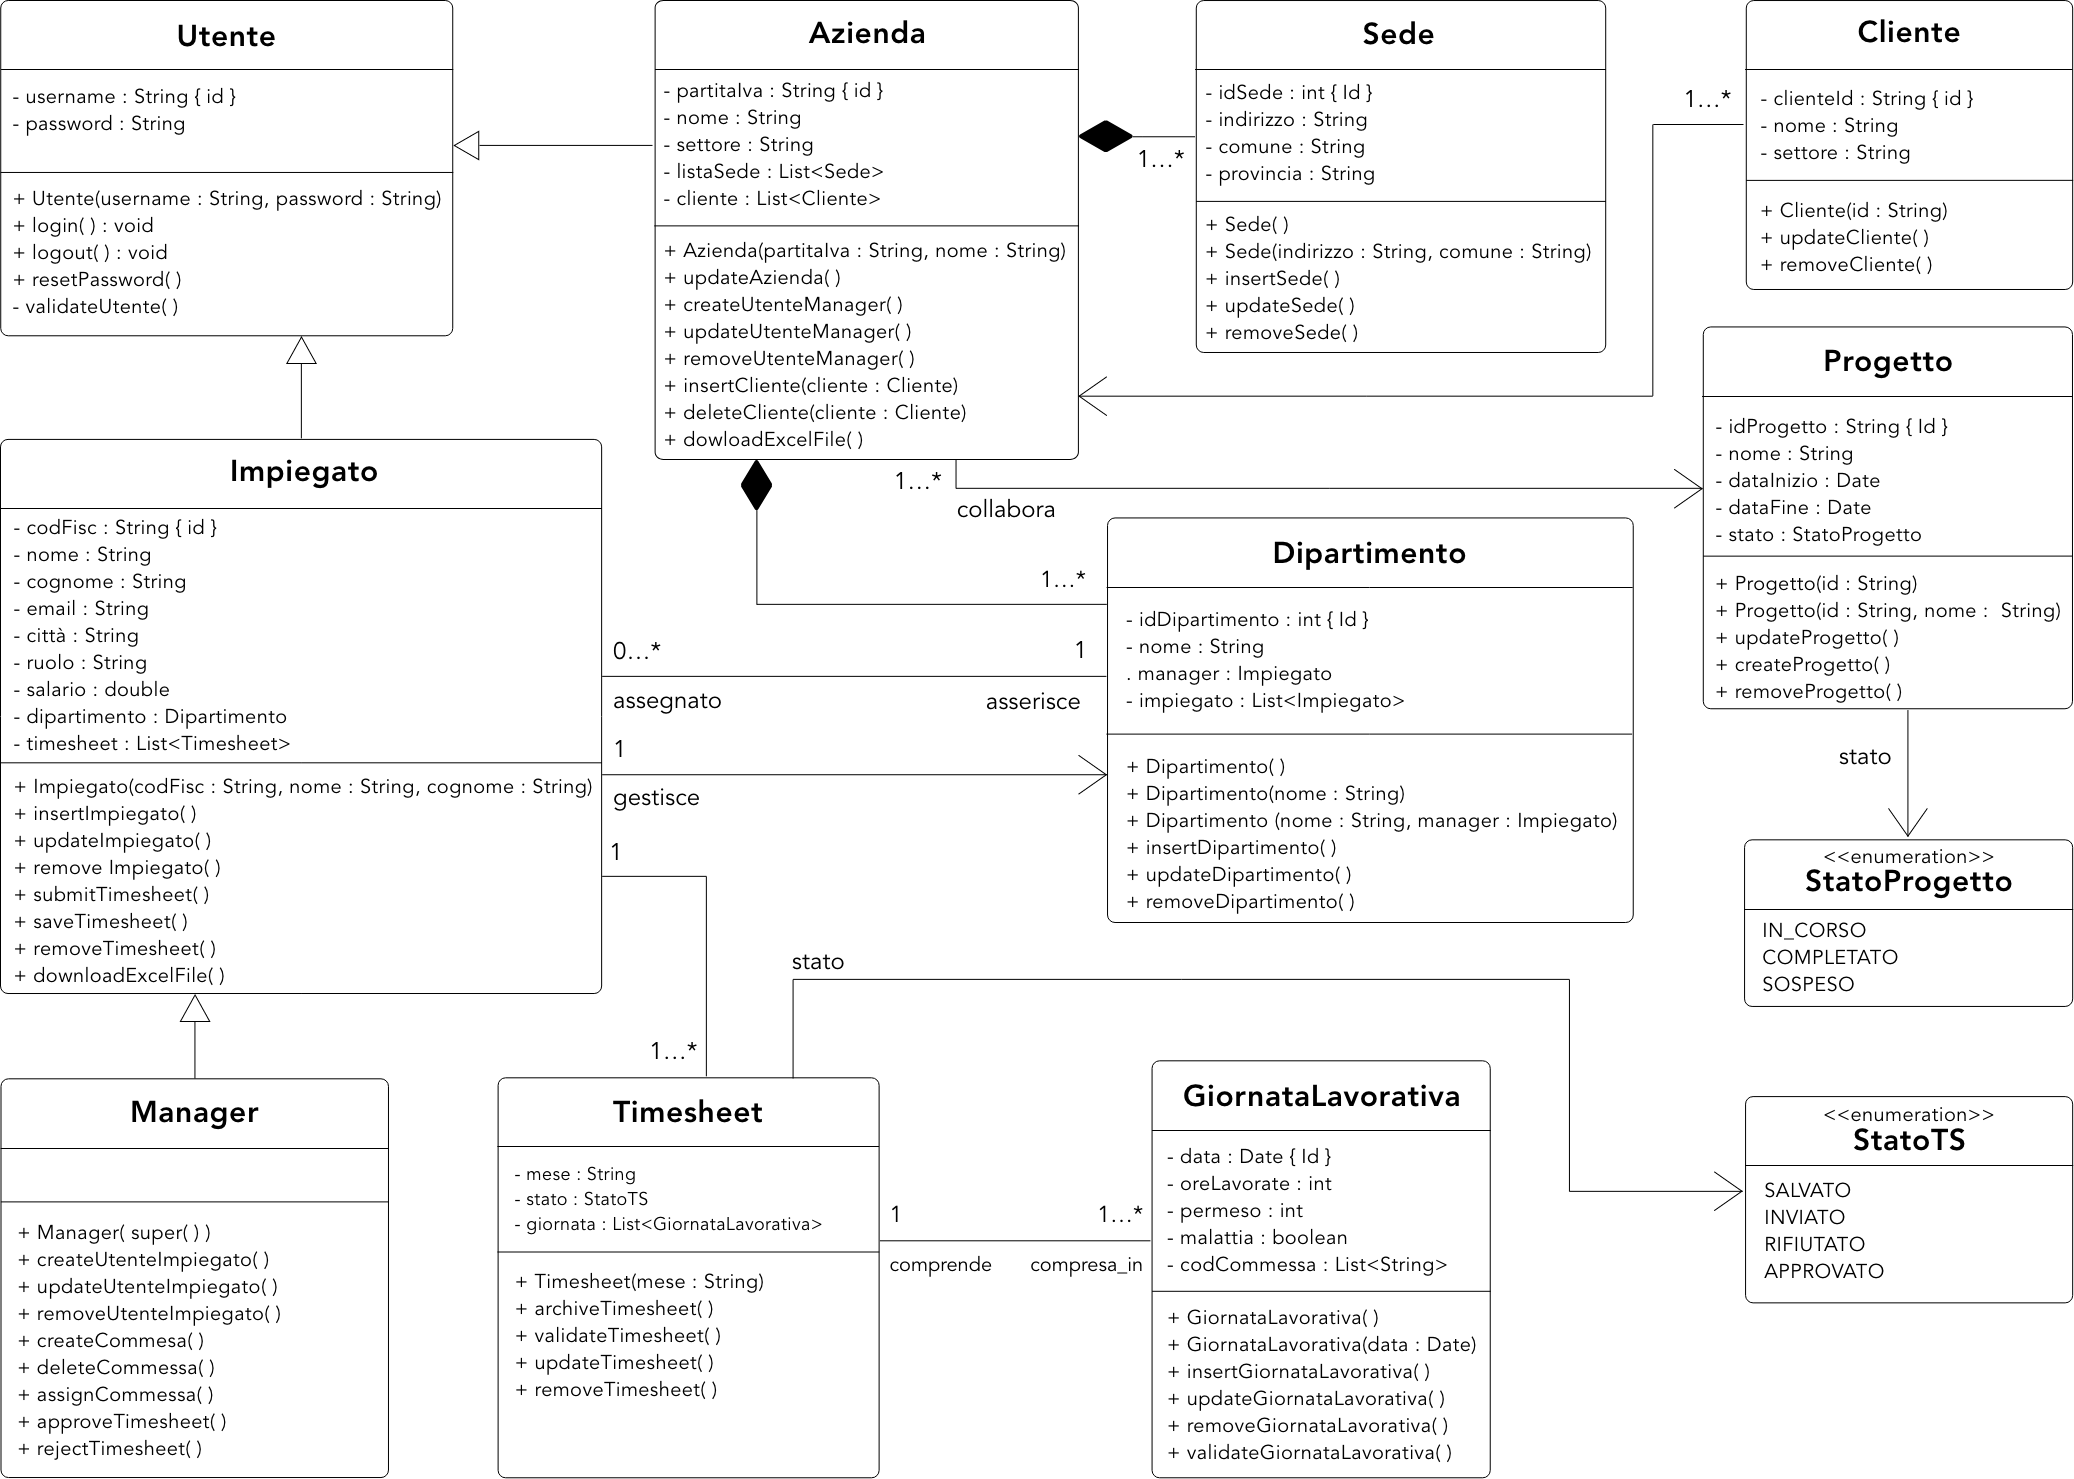
\includegraphics[width=1.3\textwidth, angle=90]{cd.png}
	\caption{Diagramma delle classi.}	
	\label{fig:cd}
\end{figure}

\clearpage
\section{Progettazione della base dati}
Durante questa fase sono state individuate in primo luogo le entità fondamentali in funzione di quanto emerso nell'analisi dei requisiti. Dunque è stato costruito un diagramma \textit{Entità-Relazione}, il quale rappresenta uno schema concettuale costituito da una serie di costrutti atti a descrivere il dominio preso in considerazione. Specificamente, i rettangoli rappresentano le \textit{entità}, ossia una classe di oggetti del mondo reale (materiali o immateriali), e ognuna di esse possiede degli attributi significativi; i rombi invece, rappresentano una \textit{relazione}, o associazione, la quale è caratterizzata da un nome (e da eventuali attributi se necessari) e che definisce un legame logico tra due o più entità.\\
Le entità individuate e le rispettive relazioni fra esse, vengono presentate in figura \ref{fig:er}.

\begin{figure}[H]
	\centering
	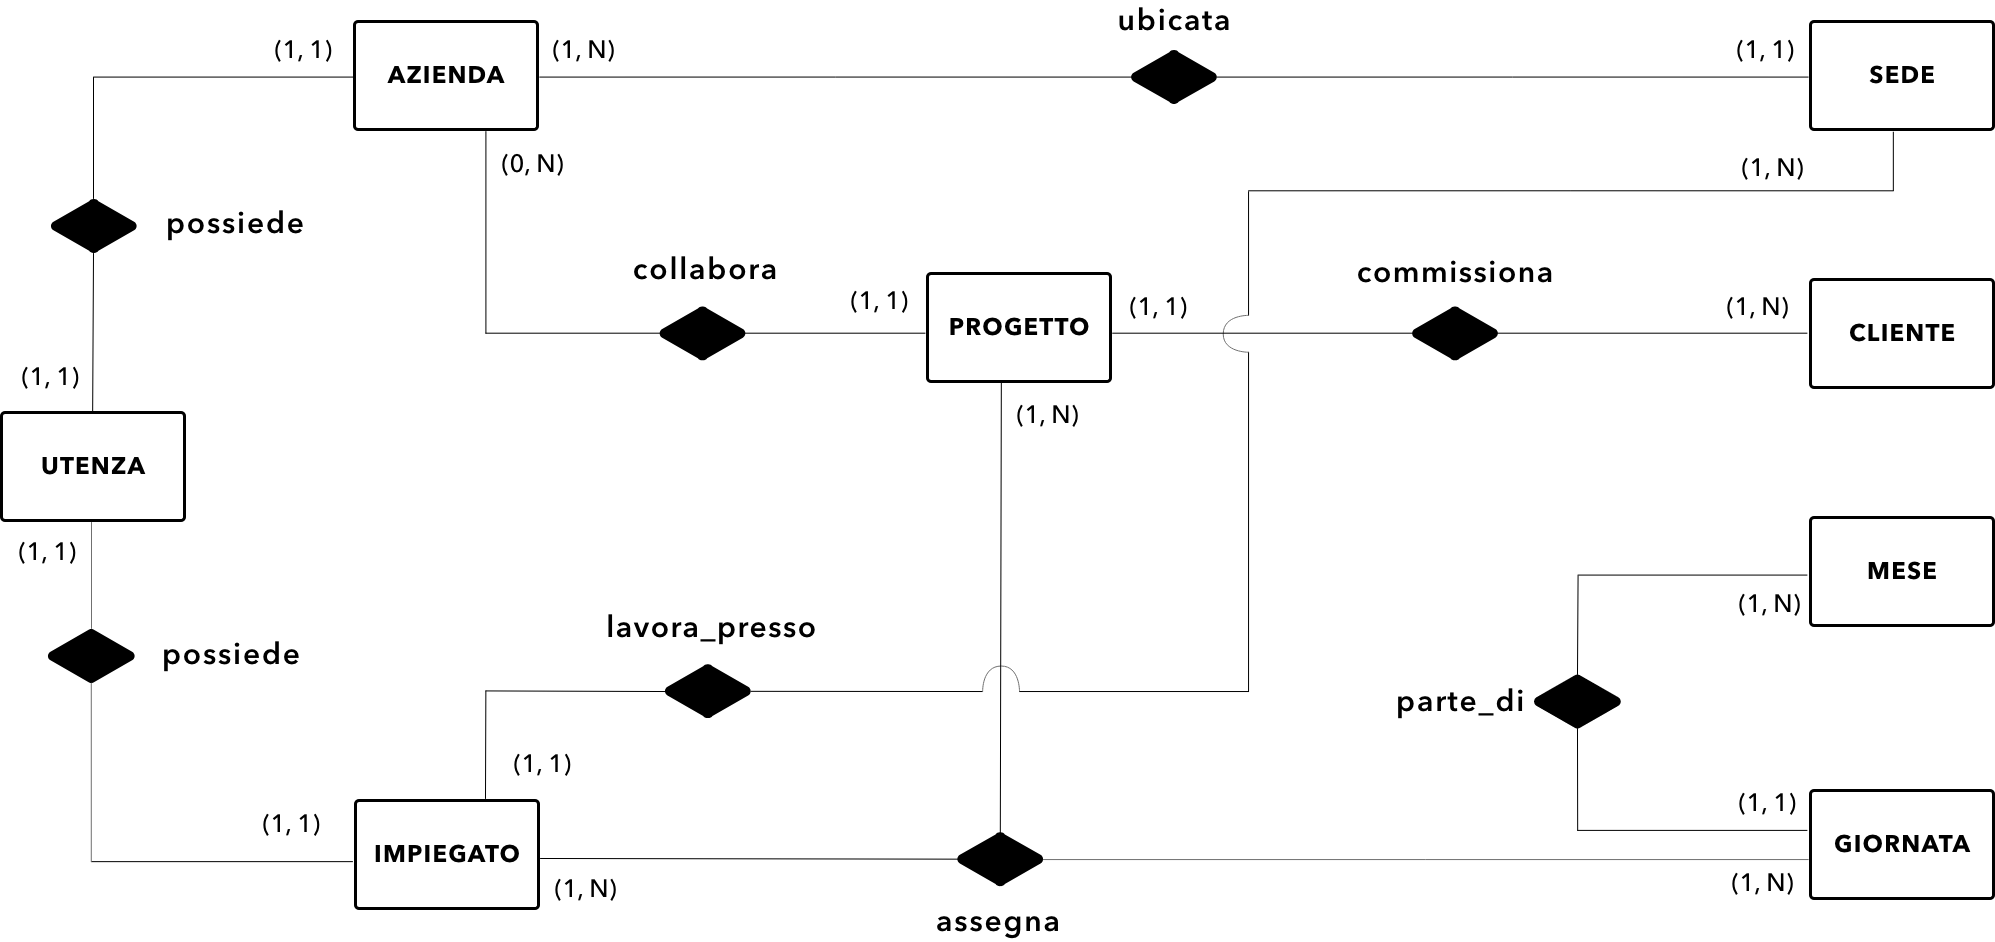
\includegraphics[width=1\textwidth]{er.png}
	\caption{Diagramma E-R della base dati.}	
	\label{fig:er}
\end{figure}

\noindent 
Successivamente, il diagramma E-R è stato tradotto in \textit{modello relazionale}, ossia uno schema logico, dove il costrutto di base è la \textit{relazione}, corrispondente ad una tabella della base dati. Per ogni relazione, o tabella, le informazioni vengono rappresentate per mezzo di tuple (righe di una tabella), le quali a loro volta sono formate da un insieme di attributi (colonne della tabella) che descrivono la relazione.\\
Di seguito, in figura \ref{fig:mod_rel}, viene presentato un diagramma che raffigura le tabelle che costituisco la base dati dell'applicazione oggetto di questa relazione.

\begin{figure}[H]
	\centering
	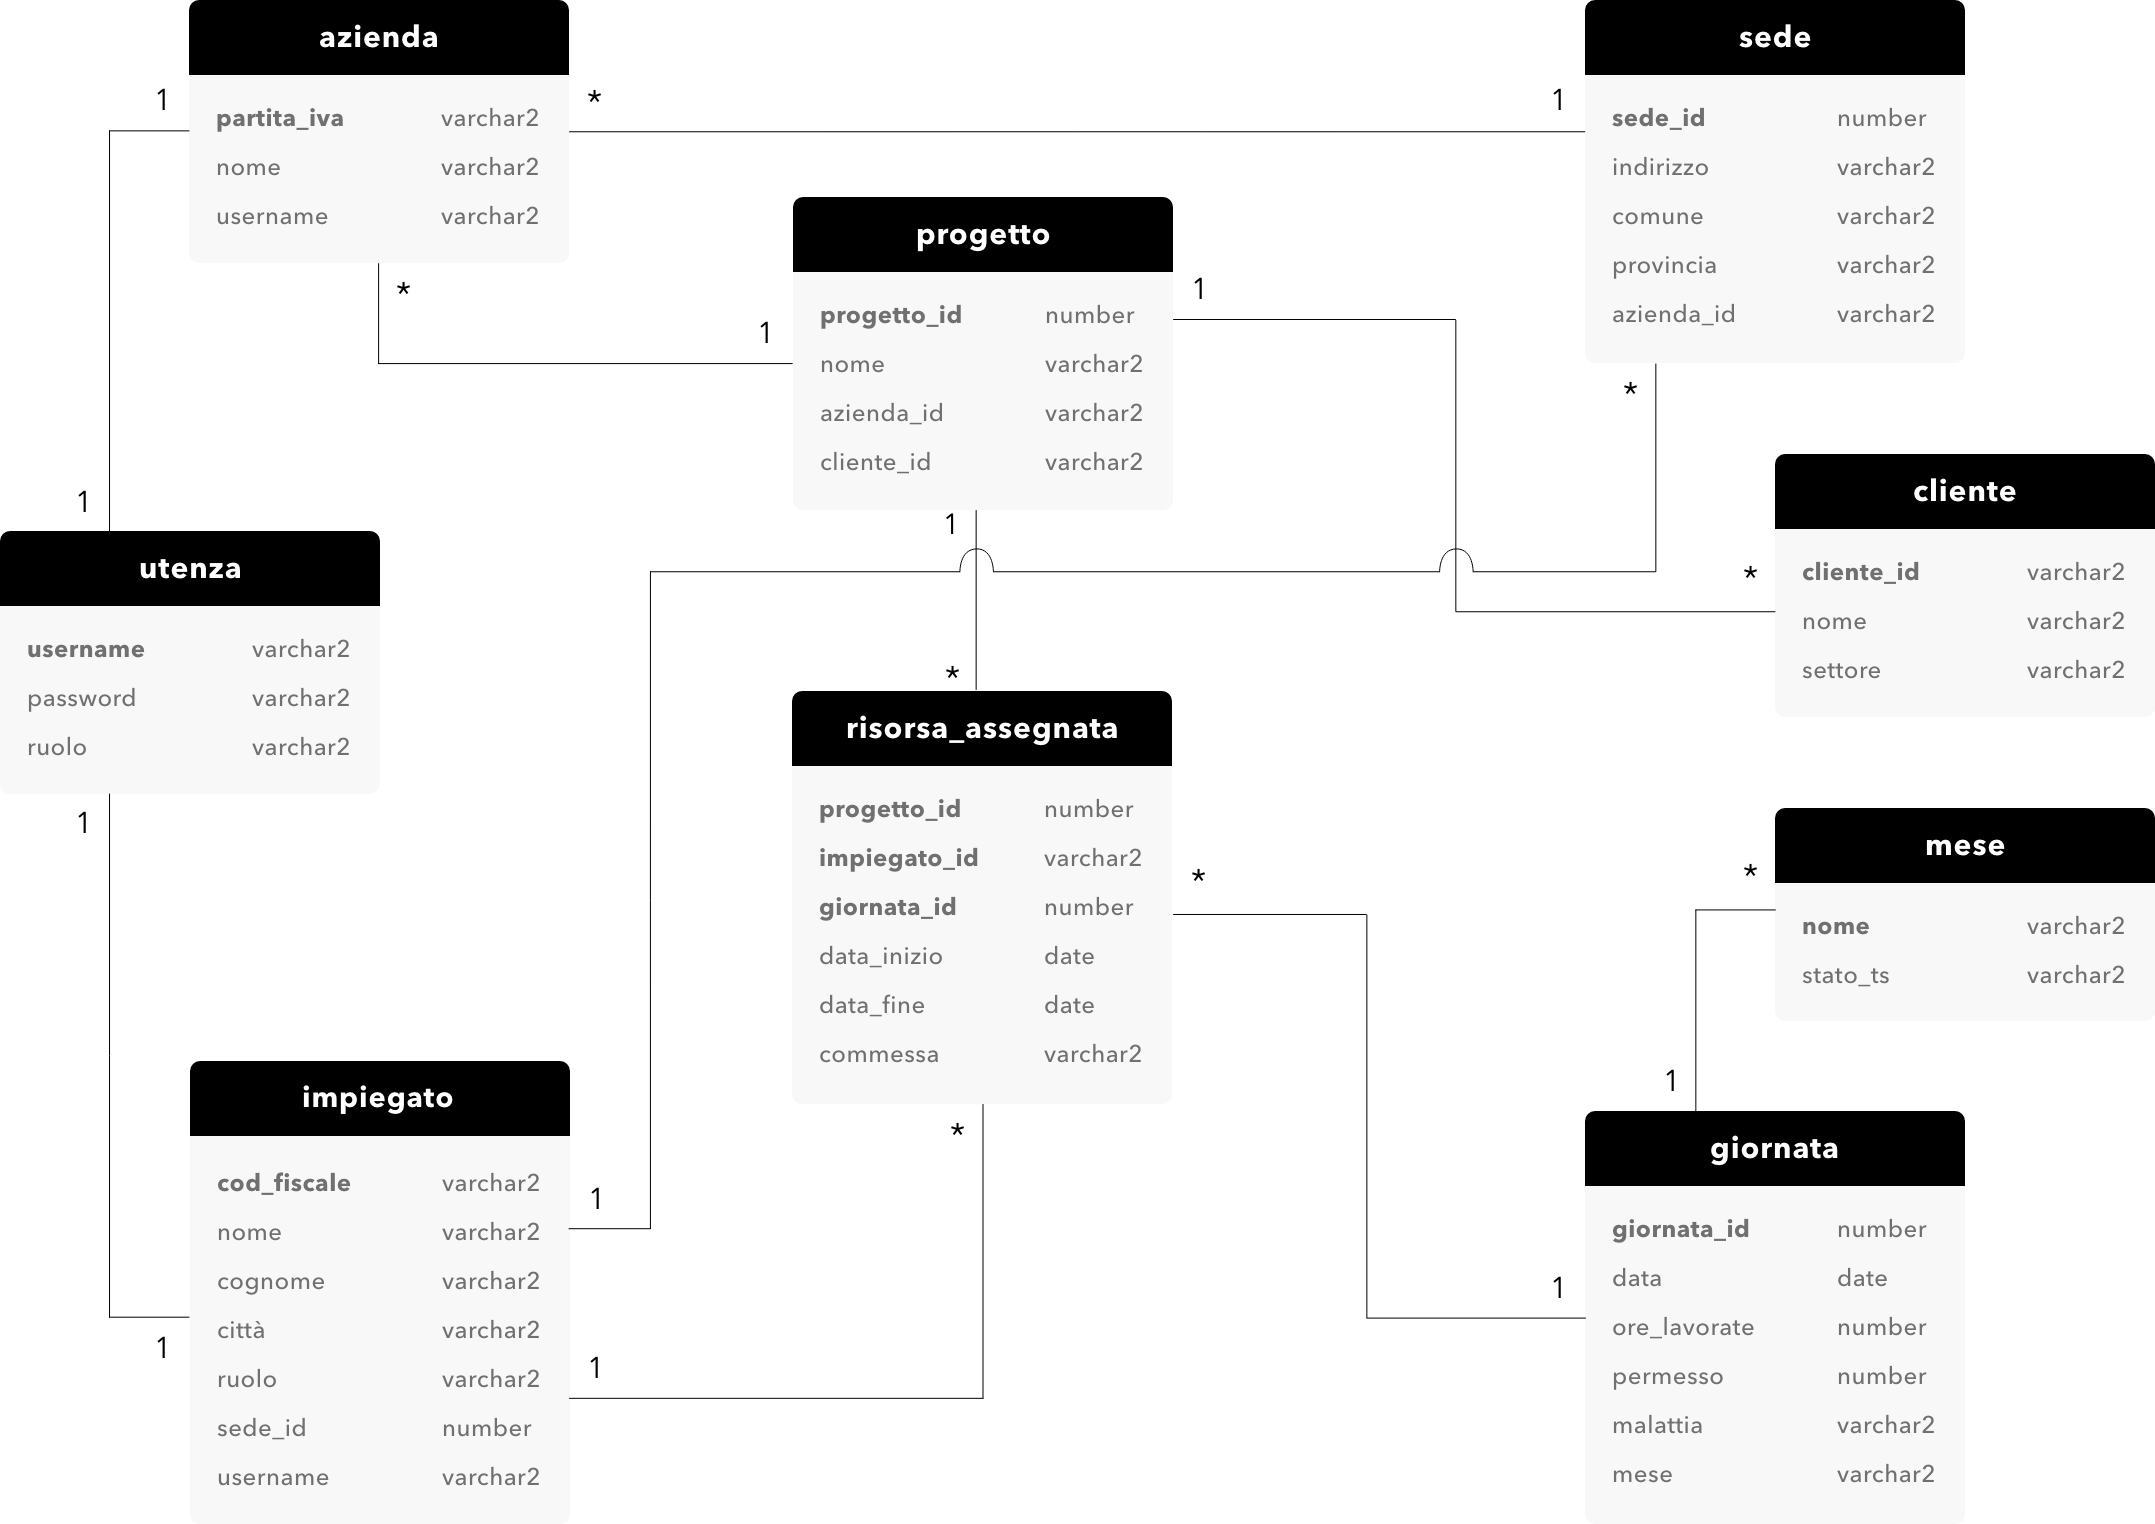
\includegraphics[width=1.4\textwidth, angle=90]{mod_rel.png}
	\caption{Diagramma delle tabelle che costituiscono la base dati.}	
	\label{fig:mod_rel}
\end{figure}

Per la creazione delle tabelle è stato usato il linguaggio SQL. Nello specifico è stato creato uno script con tutte le istruzioni di DDL (\textit{Data Definition Language}) necessarie per la creazione delle tabelle e per l'assegnamento dei vincoli di integrità. Di seguito uno estratto di tale script:

\lstset{basicstyle=\ttfamily\footnotesize,breaklines=true}
\begin{lstlisting}[language=sql]
-- creazione della tabella IMPIEGATO senza vincoli di integrita
CREATE TABLE TEMPOAPP.IMPIEGATO (
    COD_FISC        VARCHAR2    NOT NULL,
    NOME            VARCHAR2        NULL,
    COGNOME         VARCHAR2        NULL,
    CITTA           VARCHAR2        NULL,
    EMAIL           VARCHAR2        NULL,
    RUOLO           VARCHAR2        NULL,
    SEDE_ID         NUMBER          NULL,
    USERNAME        NUMBER          NULL
)
/

-- aggiunta dei vincoli di integrita alla tabella IMPIEGATO
ALTER TABLE TEMPOAPP.IMPIEGATO ADD (
    CONSTRAINT IMP_SEDE_FK
    FOREIGN KEY (SEDE_ID)           REFERENCES TEMPOAPP.SEDE(ID),
    CONSTRAINT IMP_UTENTE_FK
    FOREIGN KEY (USERNAME)          REFERENCES TEMPOAPP.UTENTE(ID),
    CONSTRAINT EMAIL_UK
    UNIQUE (EMAIL),
    CONSTRAINT COD_FISC_PK
    PRIMARY KEY (COD_FISC)
);
\end{lstlisting}

Inoltre, la macchina utilizzata per ospitare tale base dati è un \textit{Autonomous Data Warehouse} (ADW) Oracle, servizio fornito tramite cloud. Questa scelta deriva dalla necessità di avere una base dati Oracle, che fosse compatibile con il sistema operativo MacOS e che non richiedesse l'uso di una macchina virtuale eseguita in locale. Infine, per l'esecuzione degli script, e in generale per tutte le operazioni di interrogazione tramite il linguaggio SQL, è stato utilizzato il software Oracle SQL Developer.